% LTeX: enabled=false
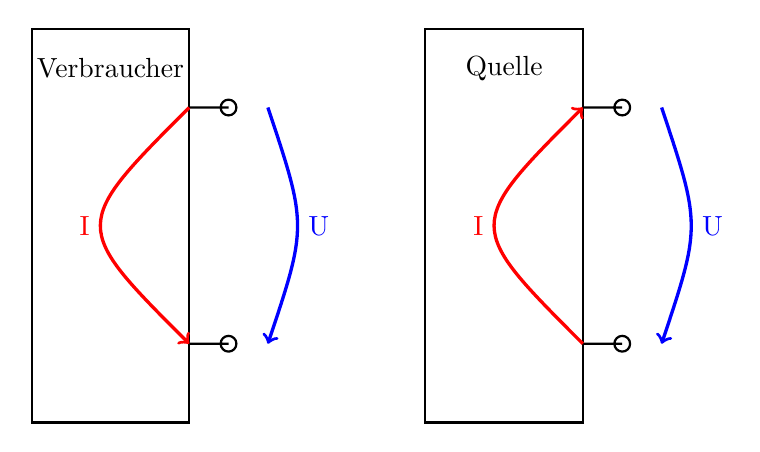
\begin{tikzpicture}
    \draw[thick] (0,0) rectangle (2,5);
    \node at (1,4.5) {Verbraucher};
    \foreach \y in {1,4}
        \draw[thick] (2,\y) -- ++(0.5,0) circle [radius=0.1];

    \draw[<-,red,very thick] (2,1) .. controls (0.5,2.5) .. (2,4) node[midway,left] {I};
    \draw[<-,blue,very thick] (3,1) .. controls (3.5,2.5) .. (3,4) node[midway,right] {U};

    \draw[thick] (5,0) rectangle (7,5);
    \node at (6,4.5) {Quelle};
    \foreach \y in {1,4}
        \draw[thick] (7,\y) -- ++(0.5,0) circle [radius=0.1];

    \draw[->,red,very thick] (7,1) .. controls (5.5,2.5) .. (7,4) node[midway,left] {I};
    \draw[<-,blue,very thick] (8,1) .. controls (8.5,2.5) .. (8,4) node[midway,right] {U};      
\end{tikzpicture}  
